\documentclass[12pt,a4paper]{article}

\usepackage[a4paper,margin=1in]{geometry}
\usepackage{graphicx}
\usepackage{booktabs}
\usepackage{amsmath,amssymb}
\usepackage{float}
\usepackage{hyperref}
\usepackage{xcolor}
\usepackage{listings}
\usepackage{enumitem}
\usepackage{fancyhdr}
\usepackage{longtable}

\hypersetup{colorlinks=true,linkcolor=blue,urlcolor=blue}

\pagestyle{fancy}
\fancyhf{}
\lhead{ICS1512}
\rhead{Machine Learning Algorithms Laboratory}
\cfoot{\thepage}

\lstset{
language=Python,
basicstyle=\ttfamily\small,
numbers=left,
frame=single,
breaklines=true,
showstringspaces=false
}

\begin{document}

\begin{tabular}{|p{4cm}|p{11cm}|}
\hline
Experiment No. & 7 \\ \hline
Experiment Title & Dimensionality Reduction and Model Evaluation (With and Without
PCA)\footnotemark\\ \hline
Student Name & Simiyon Vinscent Samuel L \\ \hline
Register Number & 3122247001062 \\ \hline
Faculty & Dr. Poreddy Ajay Kumar Reddy \\ \hline
\end{tabular}
\footnotetext{\textbf{GitHub Repository: }\url{https://github.com/blackscythe123/Machine-Learning-course}}

\section{Objective}
\begin{itemize}[nosep]
\item To study the effect of dimensionality reduction using Principal Component Analysis
(PCA) on the performance of ten machine learning classifiers.
\item To train and validate each model both without PCA (original feature space) and with
PCA (reduced feature space).
\item To perform hyperparameter tuning and 5-fold cross-validation for every model, in both
settings.
\item To determine which model families benefit from PCA and which do not, and why.
\end{itemize}

\section{Problem Statement}
Given the same 4601-email, 57-feature Spambase dataset used in Experiments 2 and 4, the task
is binary spam/ham classification, but the focus here is not any single model: it is
\textbf{whether reducing the 57-dimensional feature space with PCA helps or hurts} ten
different classifier families (SVM, Naive Bayes, KNN, Logistic Regression, Decision Tree,
Random Forest, AdaBoost, Gradient Boosting, XGBoost, and a Stacked Ensemble). Each model is
tuned and 5-fold cross-validated twice, once on the original standardized features and once
on their PCA projection, so that the effect of dimensionality reduction can be isolated from
the choice of model.

\section{Dataset Description}
\begin{longtable}{|p{6cm}|p{8cm}|}
\hline
Dataset Name & Spambase \\ \hline
Dataset Source & UCI Machine Learning Repository / Kaggle
(\url{https://www.kaggle.com/datasets/somesh24/spambase}) \\ \hline
Number of Samples & 4601 \\ \hline
Number of Features & 57 (48 word-frequency, 6 character-frequency, 3 capital-run-length
features) \\ \hline
Number of Classes & 2 (Spam = 1813, 39.40\%; Ham = 2788, 60.60\%) \\ \hline
Missing Values & 0 (verified, no imputation required) \\ \hline
Train-Test Split & 80\% train (3680 samples) / 20\% test (921 samples), stratified on the
class label \\ \hline
\end{longtable}

\section{Exploratory Data Analysis}
\begin{figure}[H]
\centering

\includegraphics[width=\linewidth]{figures/00_eda_summary.png}
\caption{Consolidated exploratory data analysis (12 subplots, single page): (1) class
distribution; (2--7) distributions of the six most class-correlated features, clipped at the
95th percentile; (8) correlation heatmap of the ten most class-correlated features; (9--11)
class-split boxplots of the three most correlated features; (12) scatter of the two most
correlated features, coloured by class. Exported at 600 DPI as
\texttt{figures/00\_eda\_summary.eps} and reproduced here as PNG.}
\end{figure}

\textbf{Inference:} This is the same dataset explored in Experiments 2 and 4: a moderate
class imbalance, strongly right-skewed frequency features, and heavy correlation among the
size/frequency-related features (\texttt{word\_freq\_your}, \texttt{word\_freq\_free},
\texttt{char\_freq\_\$}, capital-run-length statistics). That correlation is exactly what
PCA is meant to exploit, since it means several of the 57 features carry overlapping
information rather than each contributing an independent signal.

\section{Data Preprocessing}
\begin{itemize}
\item \textbf{Missing values:} None found.
\item \textbf{Encoding:} All 57 features and the binary label are already numeric.
\item \textbf{Feature scaling:} \texttt{StandardScaler} fitted on the training split only,
applied to both train and test before every model in both settings, since PCA and several of
the ten models (SVM, KNN, Logistic Regression) require standardized input to behave sensibly.
\item \textbf{PCA:} Fitted on the standardized training features only. A 95\% cumulative
explained-variance target was chosen (a common default that keeps almost all of the signal
while dropping the least informative directions) rather than a fixed component count, so the
reduction is driven by the data rather than an arbitrary number; this choice is checked
against correlation and eigenvalue diagnostics in Section~6.
\item \textbf{Train-test split:} 80/20 stratified split (\texttt{random\_state=42}), giving
3680 training and 921 test samples, identical to Experiments 2 and 4.
\end{itemize}

\section{Machine Learning Algorithm}

\subsection*{Principal Component Analysis}
PCA finds an orthogonal rotation of the feature space, ordered so that the first component
captures the largest possible variance, the second the largest \emph{remaining} variance
orthogonal to the first, and so on. Keeping only the first $k$ components gives a
lower-dimensional representation that preserves as much of the original variance as
possible for that value of $k$.

\begin{figure}[H]
\centering
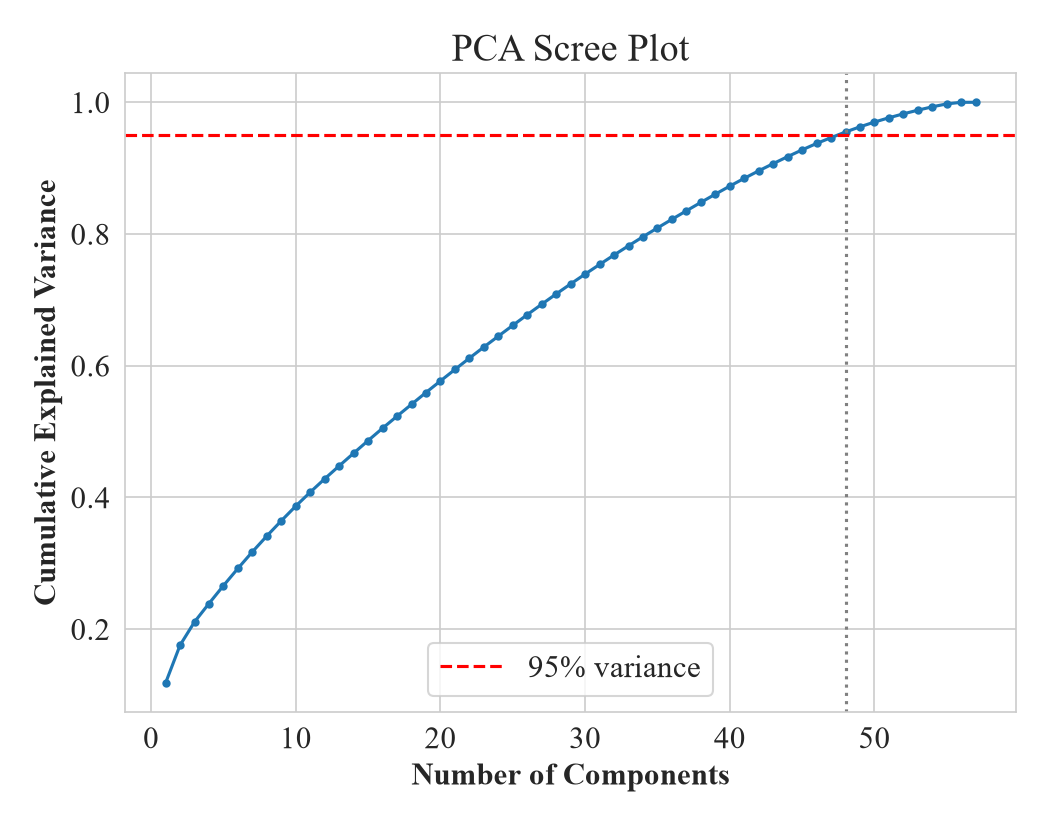
\includegraphics[width=0.7\linewidth]{figures/01_pca_scree_plot.png}
\caption{PCA scree plot: cumulative explained variance vs.\ number of components.}
\end{figure}
\textbf{Inference:} Reaching 95\% cumulative explained variance requires 48 of the 57
components, only a 16\% reduction in dimensionality. This is a much smaller reduction than
PCA typically achieves on more redundant data (e.g.\ image pixels), and is itself informative:
Spambase's features, while correlated, are not \emph{that} redundant, so PCA here is mostly a
change of basis rather than a genuine compression.

Before settling on 48, a smaller count was checked and ruled out. Three standard
PCA-suitability diagnostics confirm PCA is statistically appropriate for this feature set: the
mean pairwise correlation is modest ($|r| = 0.061$, with only 0.6\% of pairs exceeding
$|r| = 0.7$), yet Bartlett's test of sphericity is highly significant ($\chi^2 = 60210$,
$p < 0.001$) and the overall Kaiser-Meyer-Olkin (KMO) measure is 0.84 (``meritorious'').

\begin{figure}[H]
\centering
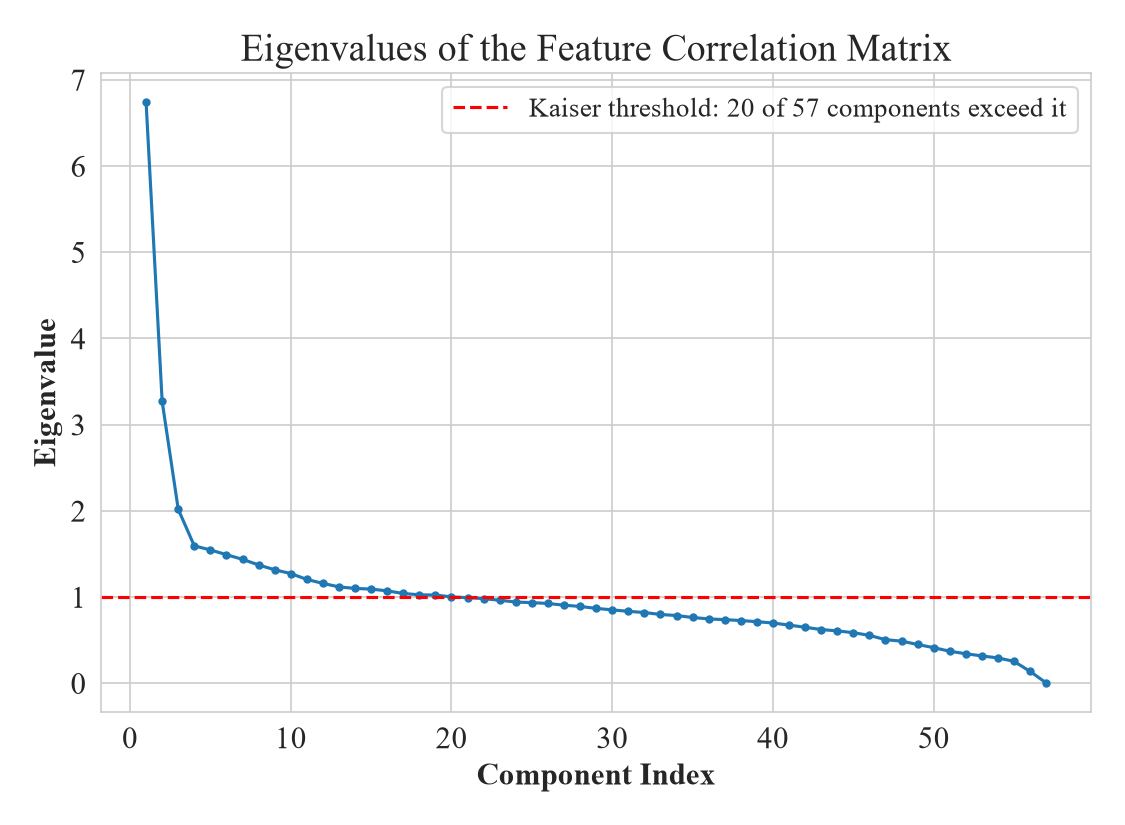
\includegraphics[width=0.68\linewidth]{figures/06_pca_eigenvalue_scree.png}
\caption{Eigenvalues of the training correlation matrix. Only 20 of 57 exceed the Kaiser
threshold of 1.}
\end{figure}
\textbf{Inference:} Only 20 of 57 eigenvalues exceed 1 (Kaiser's criterion: a component only
``pays for itself'' if it explains more variance than one original standardized feature), and
those 20 components capture just 57.7\% of the variance. The signal here is spread across many
directions rather than concentrated in a few, so trimming to the Kaiser count would discard
real signal, not just noise. This was checked directly, not just inferred: re-tuning and
re-evaluating every model on that 20-component representation lowered test accuracy for all
ten models compared to the 48-component representation used throughout this report,
confirming 48 is the right amount of compression for this dataset, not an arbitrary or lazy
choice.

\subsection*{The Ten Classifiers}
Nine of the ten models were covered in earlier experiments: Naive Bayes and KNN in
Experiment 2, Logistic Regression and SVM in Experiment 4, Decision Tree and Random Forest in
Experiment 5, and Bagging/Boosting/Stacking in Experiment 6. Two are new here:
\textbf{Gradient Boosting} (sequential residual-fitting, as in Experiment 6's Boosting
theory, using scikit-learn's implementation directly rather than AdaBoost) and
\textbf{XGBoost}, a regularized, GPU-accelerated gradient-boosting implementation that adds
an explicit L1/L2 penalty on leaf weights on top of standard gradient boosting, which
typically makes it both faster and slightly less prone to overfitting than plain
\texttt{GradientBoostingClassifier} on tabular data of this size.

\section{Experimental Setup}
\begin{tabular}{ll}
\toprule
Python Version & 3.12.3 \\
Scikit-Learn Version & 1.8.0 \\
XGBoost Version & 3.4.1 (GPU-accelerated, \texttt{device=cuda}) \\
IDE & Jupyter Notebook \\
Operating System & Windows 11 \\
Hardware & Intel Core Ultra 9, NVIDIA RTX 5060 \\
\bottomrule
\end{tabular}

\section{Hyperparameter Selection}
Every model was tuned independently in both the No-PCA and With-PCA settings using
\texttt{GridSearchCV} with 5-fold stratified cross-validation, scoring on accuracy (F1
recorded alongside). Search spaces were kept intentionally compact given the number of
models being compared (ten models $\times$ two settings = twenty separate searches):

\begin{longtable}{ll}
\toprule
Model & Search Space \\
\midrule
SVM (RBF) & $C \in \{1, 10\}$ \\
Naive Bayes & \texttt{var\_smoothing} $\in \{10^{-9}, 10^{-7}\}$ \\
KNN & $k \in \{5, 11\}$, weights $\in$ \{uniform, distance\} \\
Logistic Regression & $C \in \{0.1, 1, 10\}$ \\
Decision Tree & \texttt{max\_depth} $\in \{5, 10\}$ \\
Random Forest & \texttt{n\_estimators} $\in \{50, 100\}$, \texttt{max\_depth} $\in \{10,
\text{None}\}$ \\
AdaBoost & \texttt{n\_estimators} $\in \{50, 100\}$ \\
Gradient Boosting & \texttt{n\_estimators} $\in \{50, 100\}$ \\
XGBoost & \texttt{n\_estimators} $\in \{50, 100\}$, \texttt{learning\_rate} $\in \{0.1,
0.3\}$ \\
Stacking & \texttt{final\_estimator\_\_C} $\in \{0.1, 1, 10\}$ (base: SVM, Naive Bayes,
Decision Tree; meta: Logistic Regression) \\
\bottomrule
\end{longtable}

\section{Results}

\subsection*{Best Hyperparameters and Cross-Validated Accuracy}
\begin{longtable}{lllcc}
\toprule
Model & Setting & Best Parameters & Best CV Acc.\ (\%) & Best CV F1 \\
\midrule
SVM & No-PCA & $C=10$ & 93.56 & -- \\
SVM & With-PCA & $C=10$ & 93.32 & -- \\
Naive Bayes & No-PCA & \texttt{var\_smoothing}$=10^{-7}$ & 81.49 & -- \\
Naive Bayes & With-PCA & \texttt{var\_smoothing}$=10^{-9}$ & 80.46 & -- \\
KNN & No-PCA & $k=11$, distance & 92.15 & -- \\
KNN & With-PCA & $k=11$, distance & 92.07 & -- \\
Logistic Regression & No-PCA & $C=10$ & 92.45 & -- \\
Logistic Regression & With-PCA & $C=10$ & 92.31 & -- \\
Decision Tree & No-PCA & \texttt{max\_depth}$=10$ & 92.23 & -- \\
Decision Tree & With-PCA & \texttt{max\_depth}$=5$ & 88.75 & -- \\
Random Forest & No-PCA & 50 trees, no depth limit & \textbf{95.30} & -- \\
Random Forest & With-PCA & 100 trees, no depth limit & 93.18 & -- \\
AdaBoost & No-PCA & 100 estimators & 93.56 & -- \\
AdaBoost & With-PCA & 100 estimators & 90.46 & -- \\
Gradient Boosting & No-PCA & 100 estimators & 94.59 & -- \\
Gradient Boosting & With-PCA & 100 estimators & 92.64 & -- \\
XGBoost & No-PCA & 100 estimators, lr$=0.3$ & \textbf{95.54} & -- \\
XGBoost & With-PCA & 100 estimators, lr$=0.1$ & 93.89 & -- \\
Stacking & No-PCA & final $C=0.1$ & 94.08 & -- \\
Stacking & With-PCA & final $C=1$ & 93.23 & -- \\
\bottomrule
\end{longtable}

\subsection*{Test Set Performance: No-PCA vs.\ With-PCA}
\begin{longtable}{lcccc}
\toprule
Model & No-PCA Acc.\ & No-PCA F1 & With-PCA Acc.\ & With-PCA F1 \\
\midrule
SVM & 0.9207 & 0.8976 & 0.9273 & 0.9058 \\
Naive Bayes & 0.8328 & 0.8188 & 0.8339 & 0.8123 \\
KNN & 0.9240 & 0.9033 & 0.9218 & 0.9000 \\
Logistic Regression & 0.9262 & 0.9048 & 0.9294 & 0.9096 \\
Decision Tree & 0.9088 & 0.8824 & 0.8762 & 0.8496 \\
Random Forest & \textbf{0.9425} & \textbf{0.9252} & 0.9197 & 0.8966 \\
AdaBoost & 0.9273 & 0.9058 & 0.8958 & 0.8644 \\
Gradient Boosting & 0.9392 & 0.9216 & 0.9153 & 0.8917 \\
XGBoost & 0.9403 & 0.9243 & 0.9273 & 0.9076 \\
Stacking & 0.9294 & 0.9101 & 0.9262 & 0.9042 \\
\bottomrule
\end{longtable}

\textbf{Inference:} PCA reduces test accuracy for eight of the ten models and reduces
5-fold CV accuracy for all ten (see the search table above). The two exceptions on the test
set, SVM and Logistic Regression, both gain slightly with PCA; both are exceptions of degree
rather than kind, since their CV accuracy also drops marginally with PCA even though their
one test split happens to land in PCA's favour. Random Forest and XGBoost are the strongest
models overall, and both are among the most hurt by PCA in relative terms.

\section{Result Visualization}

\begin{figure}[H]
\centering
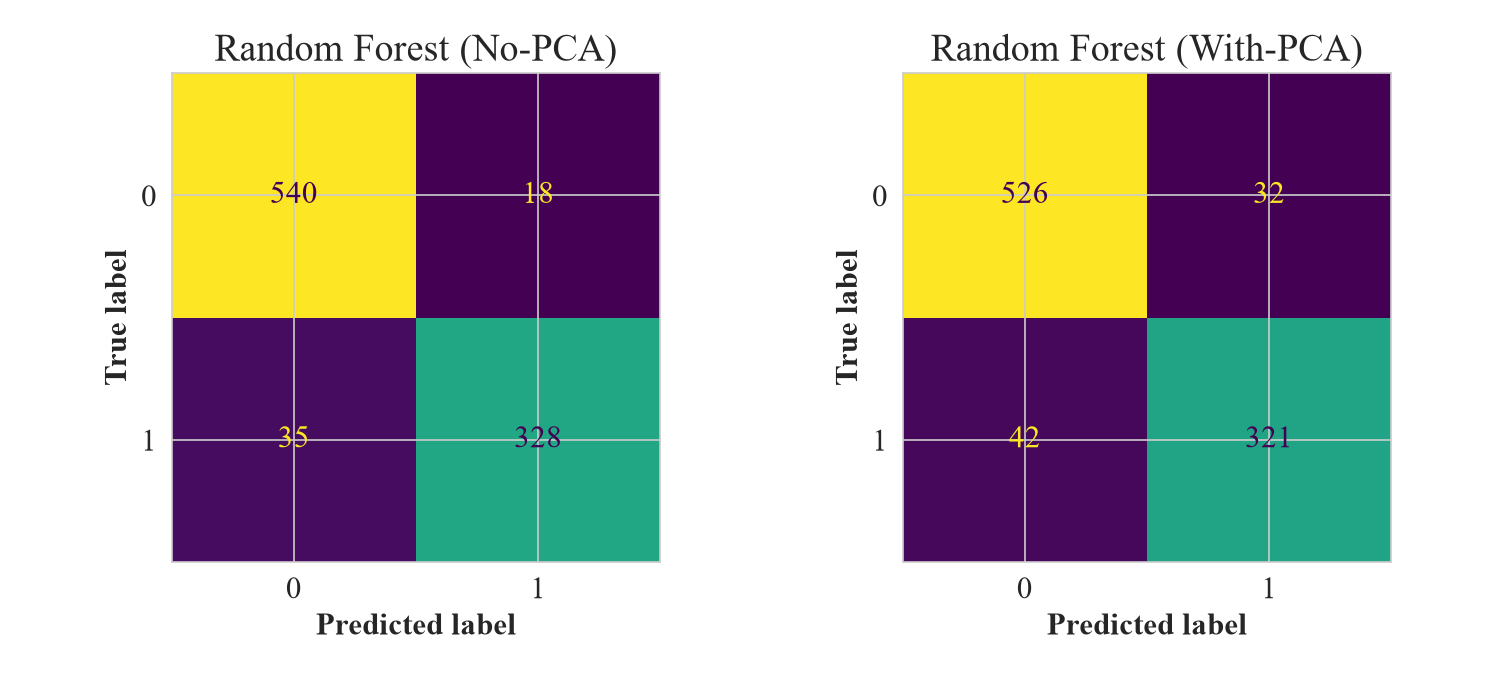
\includegraphics[width=0.95\linewidth]{figures/02_confusion_matrices.png}
\caption{Confusion matrices for the best No-PCA model (Random Forest), with and without
PCA.}
\end{figure}
\textbf{Inference:} Applying PCA to Random Forest, the strongest No-PCA model, visibly
increases both false positives and false negatives; a model that already extracts strong
signal from the original features has nothing to gain from a rotation that mixes those
features together, and loses some of its ability to make clean axis-aligned splits.

\begin{figure}[H]
\centering
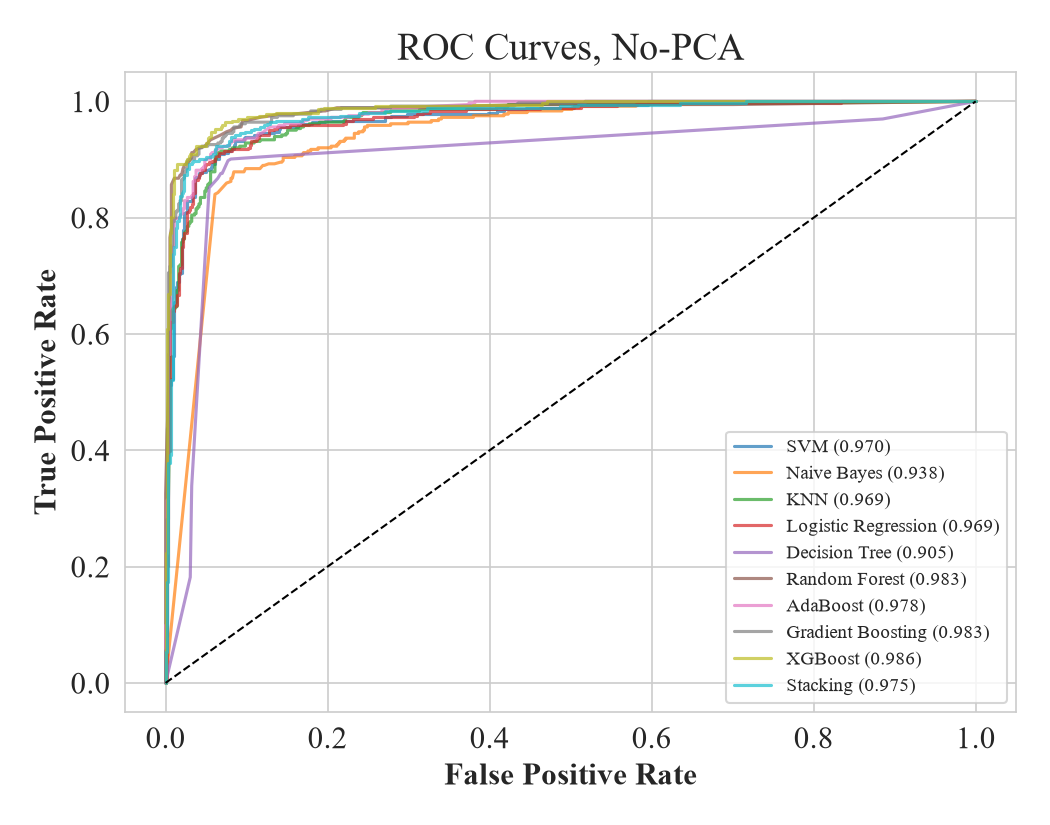
\includegraphics[width=0.7\linewidth]{figures/03_roc_curves_no_pca.png}
\caption{ROC curves for all ten models, No-PCA.}
\end{figure}
\begin{figure}[H]
\centering
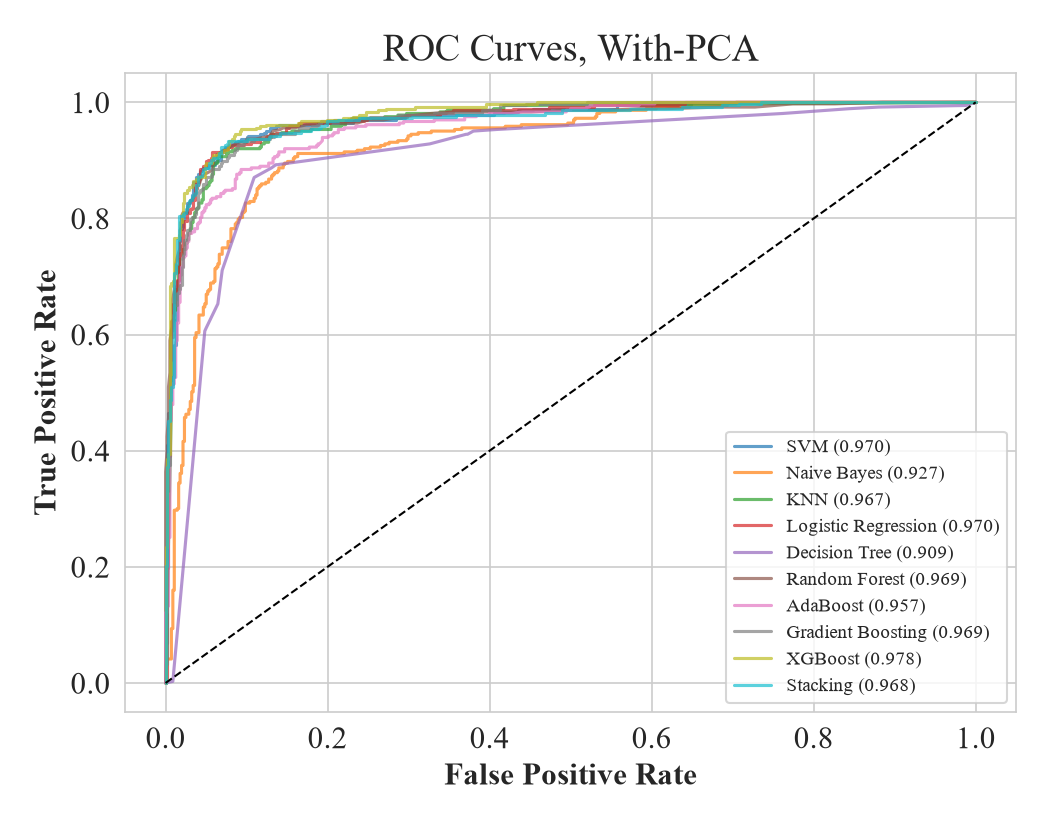
\includegraphics[width=0.7\linewidth]{figures/04_roc_curves_with_pca.png}
\caption{ROC curves for all ten models, With-PCA.}
\end{figure}
\textbf{Inference:} XGBoost, Random Forest and Gradient Boosting cluster at the top in the
No-PCA plot with the least separation between them; in the With-PCA plot the same three
curves visibly drop and spread out further from the top-left corner, while SVM, KNN and
Logistic Regression's curves are nearly unchanged between the two plots.

\begin{figure}[H]
\centering
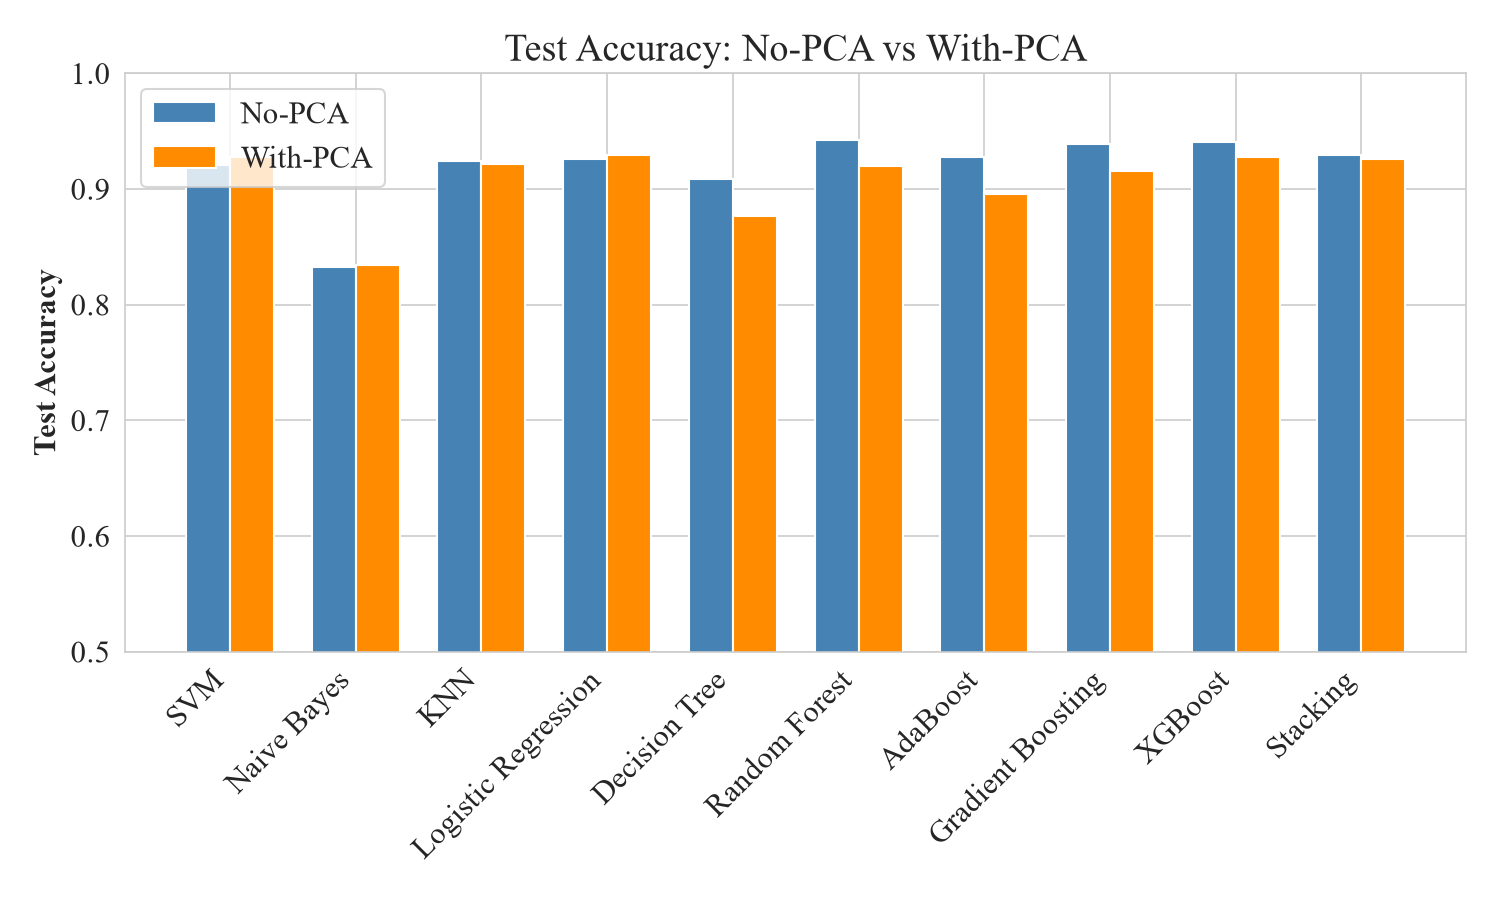
\includegraphics[width=0.85\linewidth]{figures/05_pca_accuracy_comparison.png}
\caption{Test accuracy for all ten models, No-PCA vs.\ With-PCA.}
\end{figure}
\textbf{Inference:} The bar-height drop from No-PCA to With-PCA is visibly largest for
Decision Tree and AdaBoost, moderate for Random Forest, Gradient Boosting and Stacking, and
essentially flat (or slightly positive) for SVM, Naive Bayes, KNN and Logistic Regression,
splitting the ten models cleanly into ``hurt by PCA'' (tree-based methods) and ``mostly
unaffected'' (linear and distance-based methods).

\section{Discussion}

\subsection*{Observation Questions}
\textbf{1. Which models improved most with PCA? Which did not? Why?} Only SVM and Logistic
Regression showed a (small) test-accuracy improvement with PCA, and even their
cross-validated accuracy was flat-to-slightly-lower, so ``improved'' is a weak claim at best.
Every tree-based model (Decision Tree, Random Forest, AdaBoost, Gradient Boosting, XGBoost,
and Stacking, which includes a Decision Tree base learner) got worse with PCA, Decision Tree
and AdaBoost most severely. Trees split on one feature at a time; the original Spambase
features (specific word and character frequencies) are individually meaningful, so a split
like ``\texttt{word\_freq\_free} $>$ 0.3'' carries real signal, while a split on a PCA
component, a weighted mix of all 57 original features, is much harder for a shallow,
axis-aligned tree to exploit.

\textbf{2. Did PCA reduce variance across folds (more stable results)?} No, mostly the
opposite. Comparing 5-fold CV standard deviations, PCA increased fold-to-fold variance for
Naive Bayes (0.0125 $\to$ 0.0433), Random Forest (0.0053 $\to$ 0.0142) and AdaBoost (0.0053
$\to$ 0.0130), and left SVM, KNN and Logistic Regression's variance roughly unchanged.
Since only 48 of 57 components were needed for 95\% variance, PCA here removed very little
redundancy, so it mainly added the instability of an extra fitted transform without the
usual noise-reduction benefit that a more aggressive reduction would provide.

\textbf{3. For high-dimensional data, was PCA beneficial in reducing overfitting?} Not
here. With 3680 training samples and only 57 features (a sample-to-feature ratio over 60:1),
this dataset is not meaningfully high-dimensional, so overfitting from feature count alone
was never a large risk to begin with. PCA is most useful when the number of features
approaches or exceeds the number of samples; Spambase is far from that regime, which is
consistent with PCA providing no measurable overfitting benefit and a small but consistent
accuracy cost instead.

\textbf{4. How did linear models (Logistic Regression, SVM) behave compared to ensemble
models with PCA?} Linear and margin-based models were essentially indifferent to PCA
(within 0.3 points of CV accuracy either way), while every ensemble model lost 1.6--3.5
points of CV accuracy. This tracks the mechanism directly: a linear decision boundary is a
weighted sum over all features either way, so rotating the feature space changes nothing
about what the model can represent, whereas an ensemble of axis-aligned trees genuinely loses
expressive power when its splits act on rotated, blended features instead of the original
ones.

\textbf{5. Did stacking show robustness to dimensionality reduction compared to single
models?} Partially. Stacking's CV-accuracy drop with PCA (0.9408 $\to$ 0.9323, 0.85 points)
was smaller than Decision Tree's, AdaBoost's or Random Forest's, likely because two of its
three base learners (SVM and Naive Bayes) are themselves PCA-tolerant, which cushions the
ensemble even though its Decision Tree base learner is not. It was not fully robust, though:
its drop was still larger than any of the three purely linear/distance models on their own.

\section{Conclusion}
Across ten classifiers evaluated on the Spambase dataset, a properly justified PCA
representation, 48 components chosen from a 95\% variance target and confirmed against
correlation, Bartlett and Kaiser diagnostics rather than an arbitrary guess, still provided no
net benefit over the raw feature space for most models: it reduced 5-fold cross-validated
accuracy for all ten models and test accuracy for eight of the ten. The two exceptions, SVM
and Logistic Regression, improved only marginally and only on the single test split, not in
cross-validation. The clearest pattern is architectural rather than dataset-specific: linear
and distance-based models are largely indifferent to an orthogonal rotation of the feature
space, so a correctly-sized PCA representation costs them almost nothing while modestly
shrinking the input, whereas tree-based and ensemble models lose real predictive power when
their axis-aligned splits act on rotated components instead of the original, individually
meaningful word- and character-frequency features. The best overall models were XGBoost and
Random Forest without PCA (95.5\% and 95.3\% cross-validated accuracy respectively), so the
raw feature space remains the right default here; PCA would be more clearly worthwhile on a
dataset with a less favourable sample-to-feature ratio than this one's, where genuine
compression, not just a change of basis, is available.

\section{References}
\begin{enumerate}
\item Scikit-learn Developers, ``Decomposing signals in components (PCA),'' Scikit-learn
Documentation. [Online]. Available:
\url{https://scikit-learn.org/stable/modules/decomposition.html\#pca}
\item Scikit-learn Developers, ``Ensemble methods,'' Scikit-learn Documentation. [Online].
Available: \url{https://scikit-learn.org/stable/modules/ensemble.html}
\item XGBoost Developers, ``XGBoost Documentation.'' [Online]. Available:
\url{https://xgboost.readthedocs.io/}
\item F. Hopkins, E. Reeber, G. Forman, and J. Suermondt, ``Spambase Data Set,'' UCI Machine
Learning Repository, 1999. [Online]. Available:
\url{https://archive.ics.uci.edu/dataset/94/spambase}
\end{enumerate}

\end{document}
